\section{Mechanisms of Bioprosthetic heart valve fatigue and failure}

    The mechanisms of limiting the durability of BHV can be divided into two categories: mineralization and Mechanical fatigue \cite{schoen_tissue_1999,schoen_pathology_2001,schoen_calcification_2005}. Tissue calcification primarily initiates from devitalized residual cells, usually from glutaraldehyde pretreatment \cite{schoen_calcification_2005}. Mineralization occur due to interactions between the cell membrane phosphates and the calcium within the extracellular fluids. Mechanical stress appears to accelerate calcification, but mineralization and also occur in the absence of mechanical stress. 
    To some extent, mineralization and calcification are interdependent processes \cite{sacks_collagen_2002}. Evidence suggests that mechanical deformation, either dynamic or static, potentiates mineralization but the mechanisms are unclear \cite{schoen_tissue_1999}. High levels of calcification have been generally reported to coincide with regions of high flexure, especially the commissures and basal attachment margin \cite{thubrikar_aortic_1990,schoen_pathology_2001}. It is postulated that disruption of the collagen structure may produce new nucleation sites for calcific crystals, promoting mineral growth, or simply allow fluid insudation leading to exposure to greater amounts of calcium and phosphorus ions \cite{schoen_tissue_1999}. Conversely, mechanical damage could result from direct fatigue effects, stress concentrations within the cusp induced by calcification, or direct structural damage induced by calcification \cite{schoen_calcification_2005}. Many BHVs fail with little or no calcification \cite{schoen_tissue_1999,schoen_anatomic_1985,schoen_pathology_2001}. In the study by Sacks and Schoen, it was observed that regions with disruptions in collagen fiber architecture did not necessary correspond with regions with high calcification (Fig. \ref{c1:fig:calcificationdamage}) \cite{sacks_collagen_2002}. Thus, calcification independent could be equally important mechanisms for BHV failure .
    
%-------------------	begin FIGURE 	-------------------%
\begin{figure}
\centering
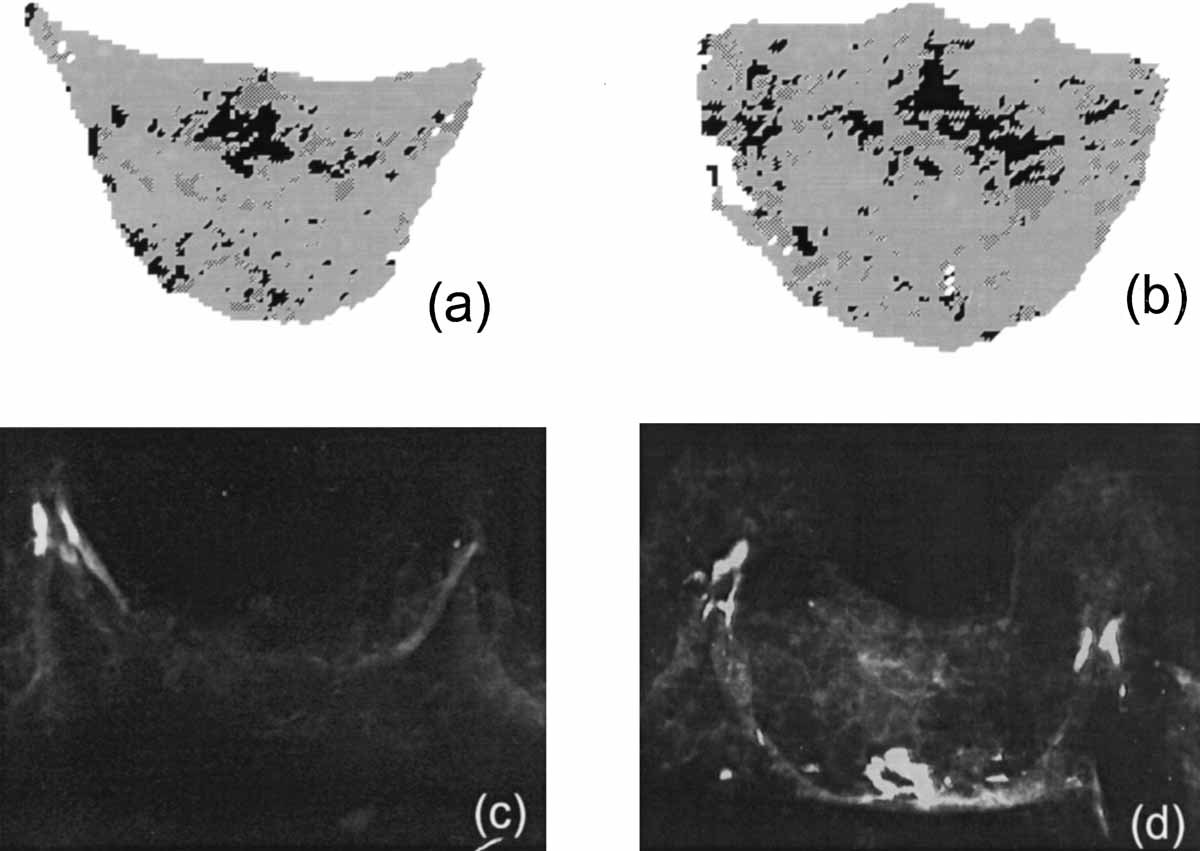
\includegraphics[width=5.0in]{Images/chapter1/calcificationdamage.jpg}
\caption{(a,b) Regions of collagen fiber damage derived from SALS data by plotting regions with large distruptions in collagen fiber structure in black. (c,d) Corresponding X‐ray photos showing pronounced calcification along the commissure and basal attachment. In both cusps regions of structural damage did not spatially correlate with regions of calcification. As shown in (e), this lack of correlation was consistent in all explanted cusps. (Adapted from \cite{sacks_collagen_2002})}
\label{c1:fig:calcificationdamage}
\end{figure}
%-------------------	 end FIGURE 	-------------------%



    Damage initially accumulates in the collagen fiber architecture (CFA) (Fig. \ref{c1:fig:damageprocess}) which in turn lead to tearing and delamination \cite{vyavahare_mechanisms_1999}. Predicting tearing and delamination (fracturing) is an extremely complex process even for solid materials without biological factors. Before tackling this, a solid groundwork of the processes that lead to this failure is needed. For BHVs this can be done by predicting the accumulation of collagen fiber damage, which leads to the development of micro-tears in the extracellular matrix (ECM) before propagating to full tissue-scale tearing. Thus, simulating fiber-level damage can be used to form preliminary estimation of BHV durability. 

\begin{figure}[hbt]
\centering
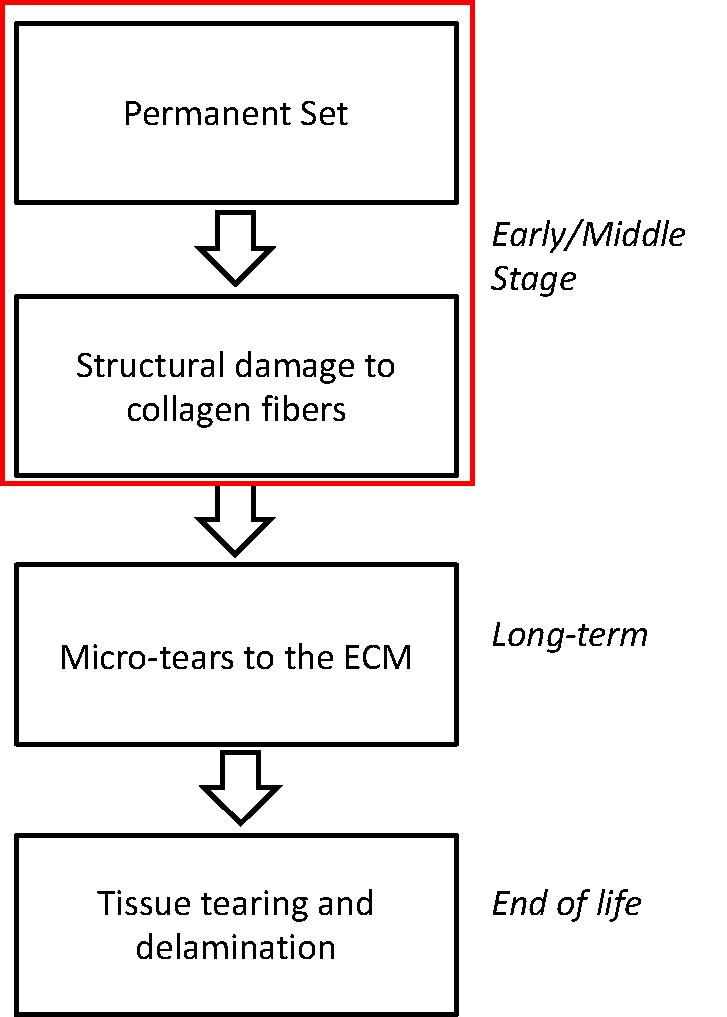
\includegraphics[width=2.75in]{Images/chapter1/damageprocess.pdf}
\caption{Stages of fatigue and failure. We will focus on the early and mid-term (Red).}
\label{c1:fig:damageprocess}
\end{figure}

    The most significant change in response to cyclic loading is the change in geometry of the BHV leaflets. In a study on the porcine aortic BHVs \cite{smith_high_1997},  Smith \textit{et al}. found significant changes in the unloaded geometry of BHVs after AWT, especially in the belly region of the leaflets (Fig. \ref{c1:fig:PSeffects}A). By changing the unloaded reference configuration, the shape of the leaflets and their mechanical response will change as well. Further analysis shown that significant structure damage occurred within the belly region as compared to other regions of the leaflet, where the stress significantly increased \cite{smith_fatigue_1999}. Interestingly, Smith et al. also found most the most significant changes in BHV leaflet geometry to occur within first 50 million cycles \cite{smith_high_1997}. Moreover, Sacks and Smith \cite{sacks_effects_1998} also found that there were minimal structural damage in this early stage (Fig. \ref{c1:fig:PSeffects}B). This is further supported by another study by Wells \textit{et al} \cite{wells_cyclic_2005}, where they found minimal structural changes during the first 50 million cycles for the pressure fixed BHVs, with most significant change observed in the first million cycles. Clearly, there is a non-damage based mechanism at play that changes the geometry of the material, with significant impact on the early stage of cycling and the rate of fatigue in later stages. 


\begin{figure}[hbt]
\centering
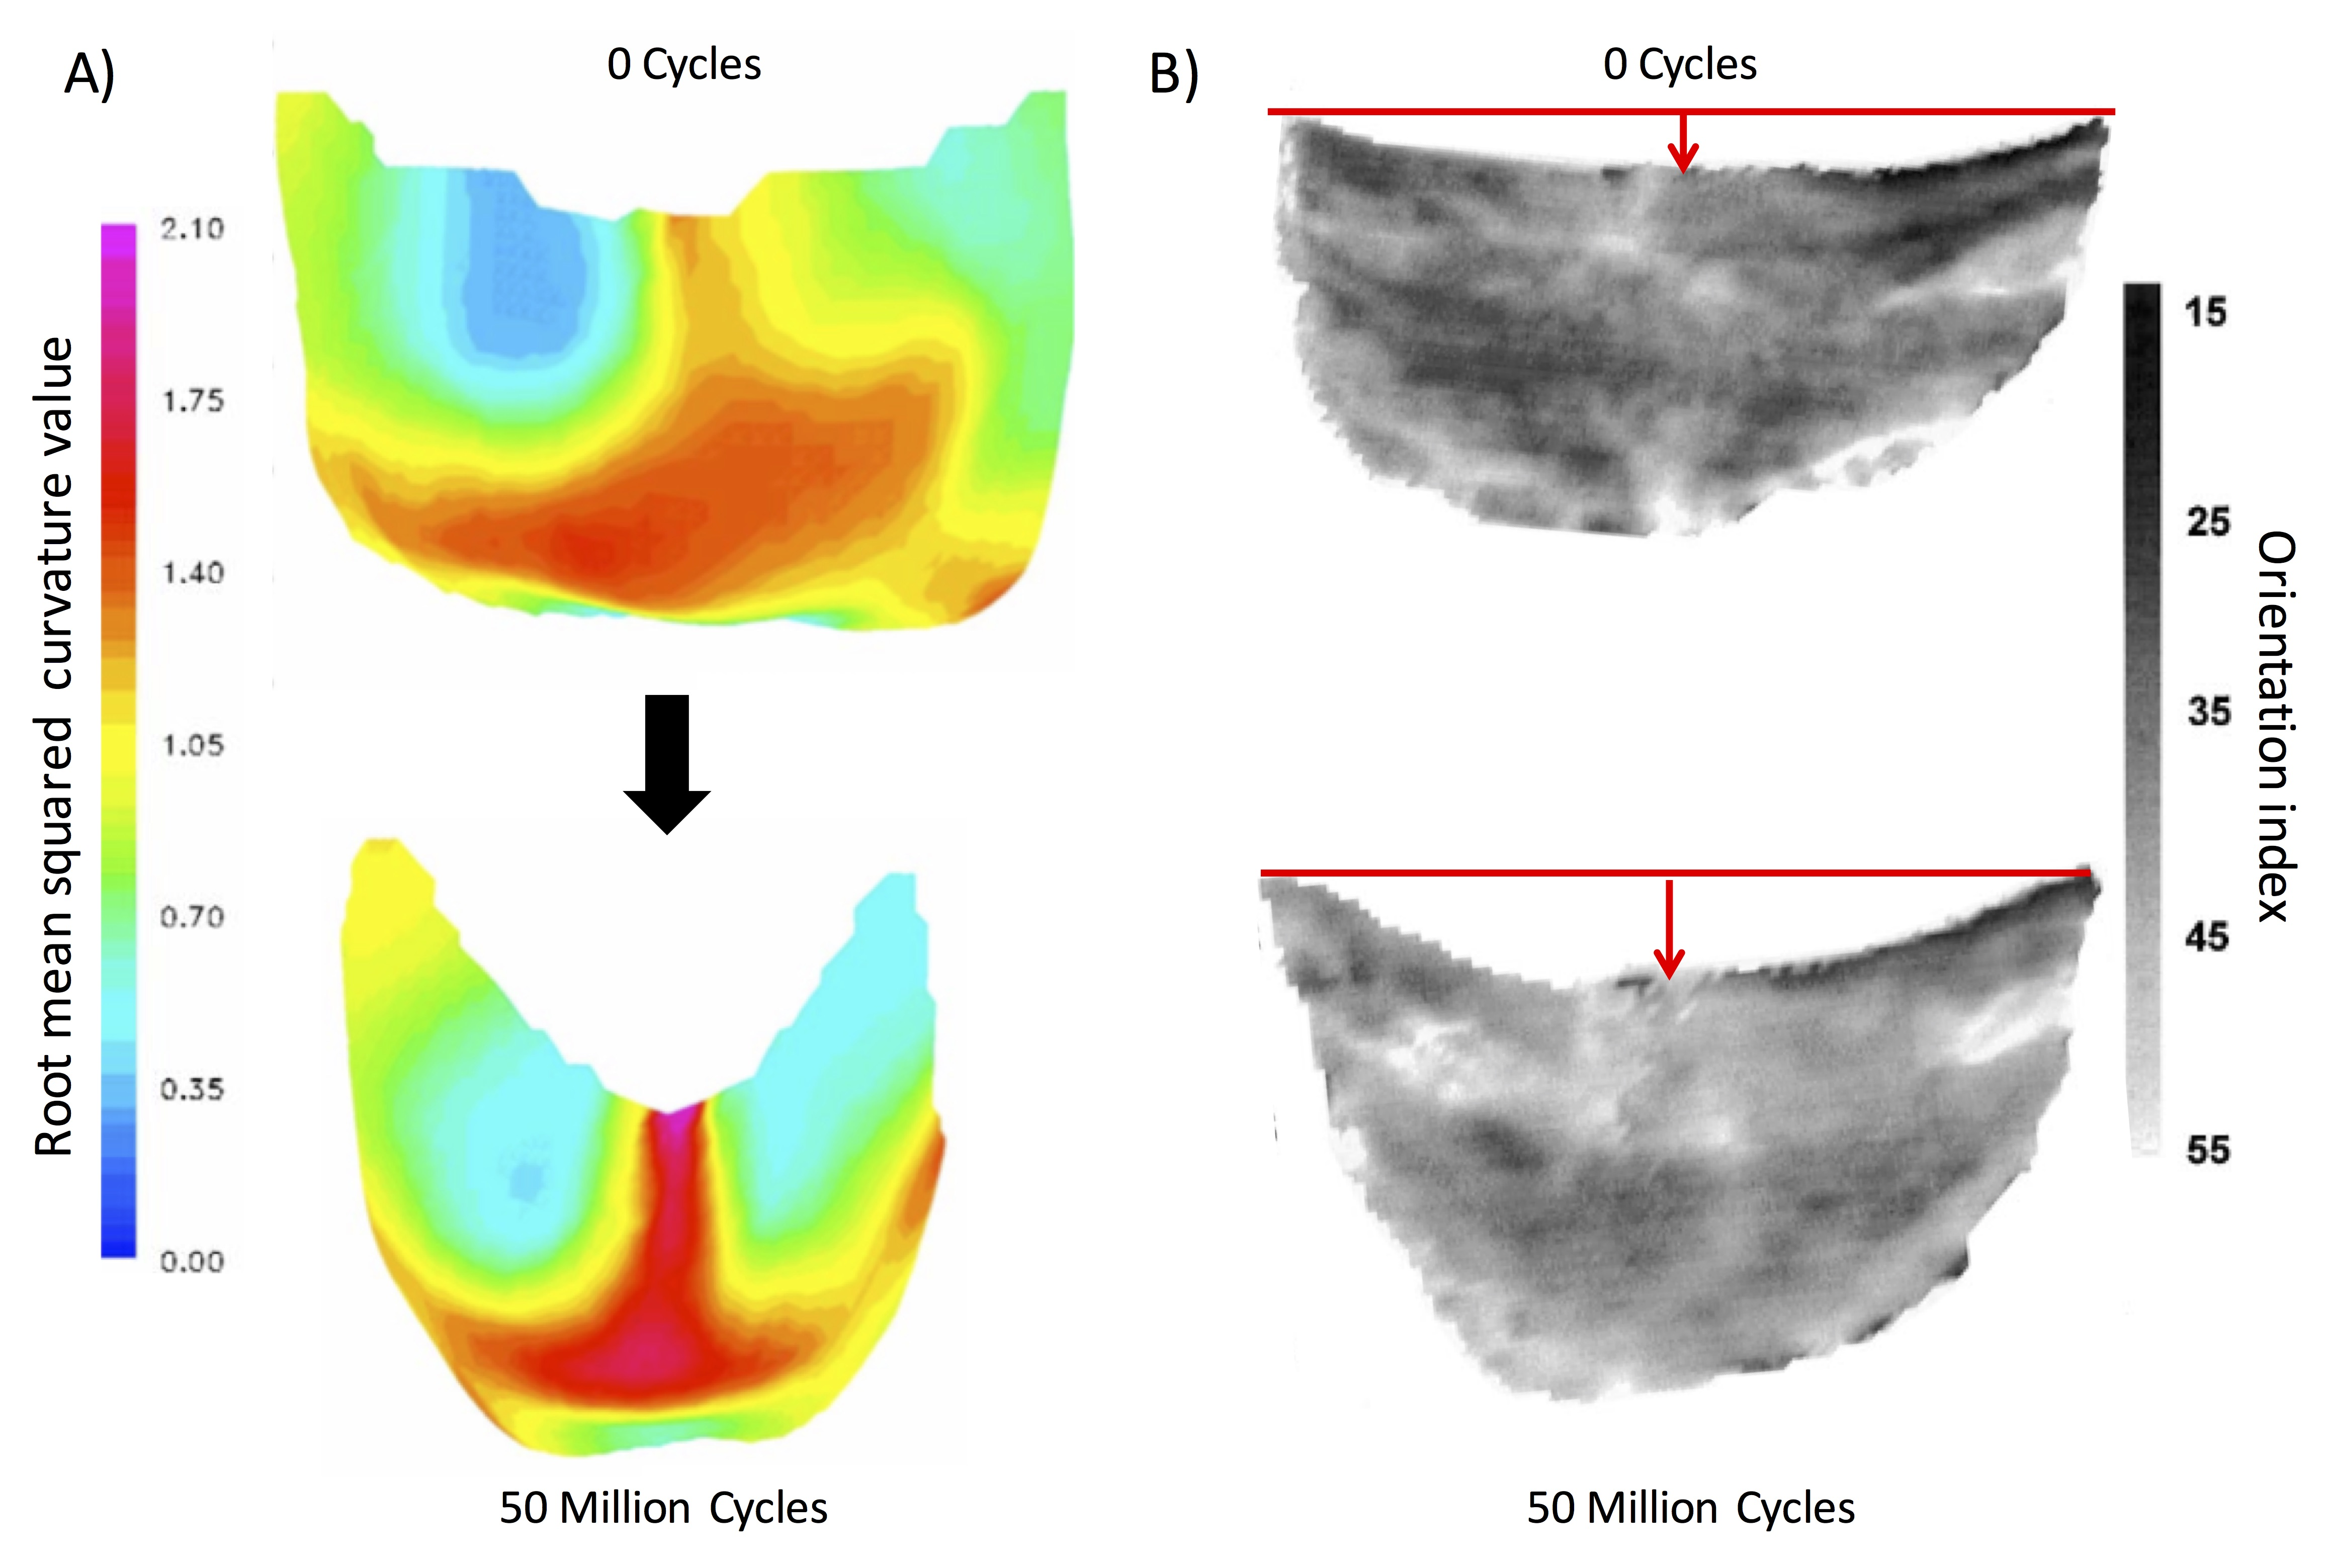
\includegraphics[width=\textwidth]{Images/chapter4/figure1}
\caption{A) The 3D unloaded geometry a BHV leaflet before and after cyclic loading, with the color indicating the local root mean squared curvature. The most significant change in geometry is in the belly region. B) BHV leaflet collagen fiber architecture, showing that the collagen fiber architecture are convected by the dimensional changes. The grayscale scale bar shows the orientation index (OI), which is angle containing 50 \% of fibers. The lack of changes in the OI suggests that minimal damage to the collagen fiber architecture has occurred.}
\label{c1:fig:PSeffects}
\end{figure}



    
